\section{History}

    1978 Turing Award winner, John Backus, used his acceptance speech to ask the
question: ``Can Programming be liberated from the von Neumann Style?''
\cite{HistoryOfHaskell}. The crux of his argument was that the traditional
and ubiquitous architecture of the day was not suitable for the eventual shift
to parallelism and the performance gains that could be achieved through
parallelism's use. This fed the
interest in novel computer architectures that would more readily support
parallelism. 
 
    Work had already been carried out on non-von Neumann architectures
before that time, however, much of it was in the form of abstract machines
that functioned `on top' of the von Neumann architecture \cite{turnerHistory}.
    In the early 70's the idea of graph reduction is introduced
(Wadsworth)\cite{wadsworth} and
with it, the concept of lazy evaluation was ready to be formalised
\cite{lazyCons, HistoryOfHaskell}. Lazy
evaluations has its roots in papers by Henderson and Morris, and Friedman and
Wise \cite{turnerHistory}.
People began to think of ways to better implement graph reduction machines.
A big breakthrough for software reduction was Turner's SKI-Combinator reduction
scheme in 1979 \cite{turnerHistory, clackbook}. 

    In the 1980's we saw a great interest in parallel architectures for
functional languages. The two main conferences in the field were `LISP and
Functional Programming' (which was held on even years) and `Functional
Programming and Computer Architecture' (which was held on odd years).

    Several novel architectures were developed with the hopes that they could
surpass stock hardware in their performance. This line of research continued
through the 80's and into the early 90's \cite{Alice, GRIP, clackbook,
PFPAnIntro}.

    The G-Machine in '84 showed that lazy functional languages (which had always
been considered inefficient) could be implemented in an efficient manner on
stock hardware. However, the abstract machine could also be used in the
implementations of novel architectures \cite{Augustsson:LazyMLCompiler}. 

    The 1990's saw a decline in the amount of research aimed at parallel
functional programming. This was mainly due to the results from earlier research
being less successful than had been hoped (some novel architectures did see good
results, but they could not keep up with the improvements seen in the sequential
hardware sphere) \cite{PFPAnIntro, clackbook}. 

    The late 90's and the 2000's saw a resurgence in the interest in parallel
functional programming. While still constrained by the von Neumann bottleneck, 
interest in this architecture is high because of the ubiquity of multi-core in 
computers today. Generally, many of the techniques discussed earlier are used, but as virtual
machines abstracting away from the hardware architecture (Like GpH using GUM, or
GHC using STG-Machine) \cite{buckwheat, haskellSharedMem}. 


While still suffering from the von Neumann bottleneck, the
utilisation of multiple cores has been of increasing interest. This brings us to
today.

\section{Sequential Computation}
    Before diving into parallel functional programming it is important to
understand how functional programs are evaluated using sequential machines. 
The Church-Rosser Theorem gives us a profound guarantee with our functional
programs: Given a valid expression, there is only one normal form for the
expression. This is true regardless of the order of reductions carried out
(given that they are valid reductions). So given a program, there can be many
possible reduction orders that all lead to the same result. What does this mean
for sequential computation? For lazy languages, such as Haskell, this means that
there is no fear of only evaluating expressions as they are needed and
terminating with an incorrect result. There is the following caveat: while there
is \emph{only one} normal form, it is possible that there could be a reduction
order that does not terminate.  

 \subsection{$G$-Machine}
    Unlike conventional register machines, the $G$-Machine is a stack based
machine designed to perform \emph{normal order} graph reduction.
    The key point for the G-Machine \cite{Augustsson:LazyMLCompiler}
is that it extended the idea that Turner introduced
with the compilation of functional programs to SKI combinators. 
But instead of relying on pre-determined combinators, why not
utilise the high-level declarations defined by the programmer? By compiling 
code for each of these, we are able to produce
efficient code for each top-level function, whereas before we only had efficient
code for each pre-determined combinator. These top-level function definitions
were coined \emph{supercombinators} by Hughes \cite{hughes:thesis}. Each 
supercombinator must not contain any lambdas on the right-hand side. In order to 
accomplish this for the $G$-Machine, Augustsson and
Johnsson expanded on the lambda-lifting technique first outlined by Hughes
\cite{Augustsson:LazyMLCompiler, hughes:thesis}. 
    
    Each supercombinator is compiled in compiled to what is essentially a
reverse postfix notation for the right-hand side of the function definition.  
The resulting code constructs and 
\begin{figure}[h!]
  \centering
  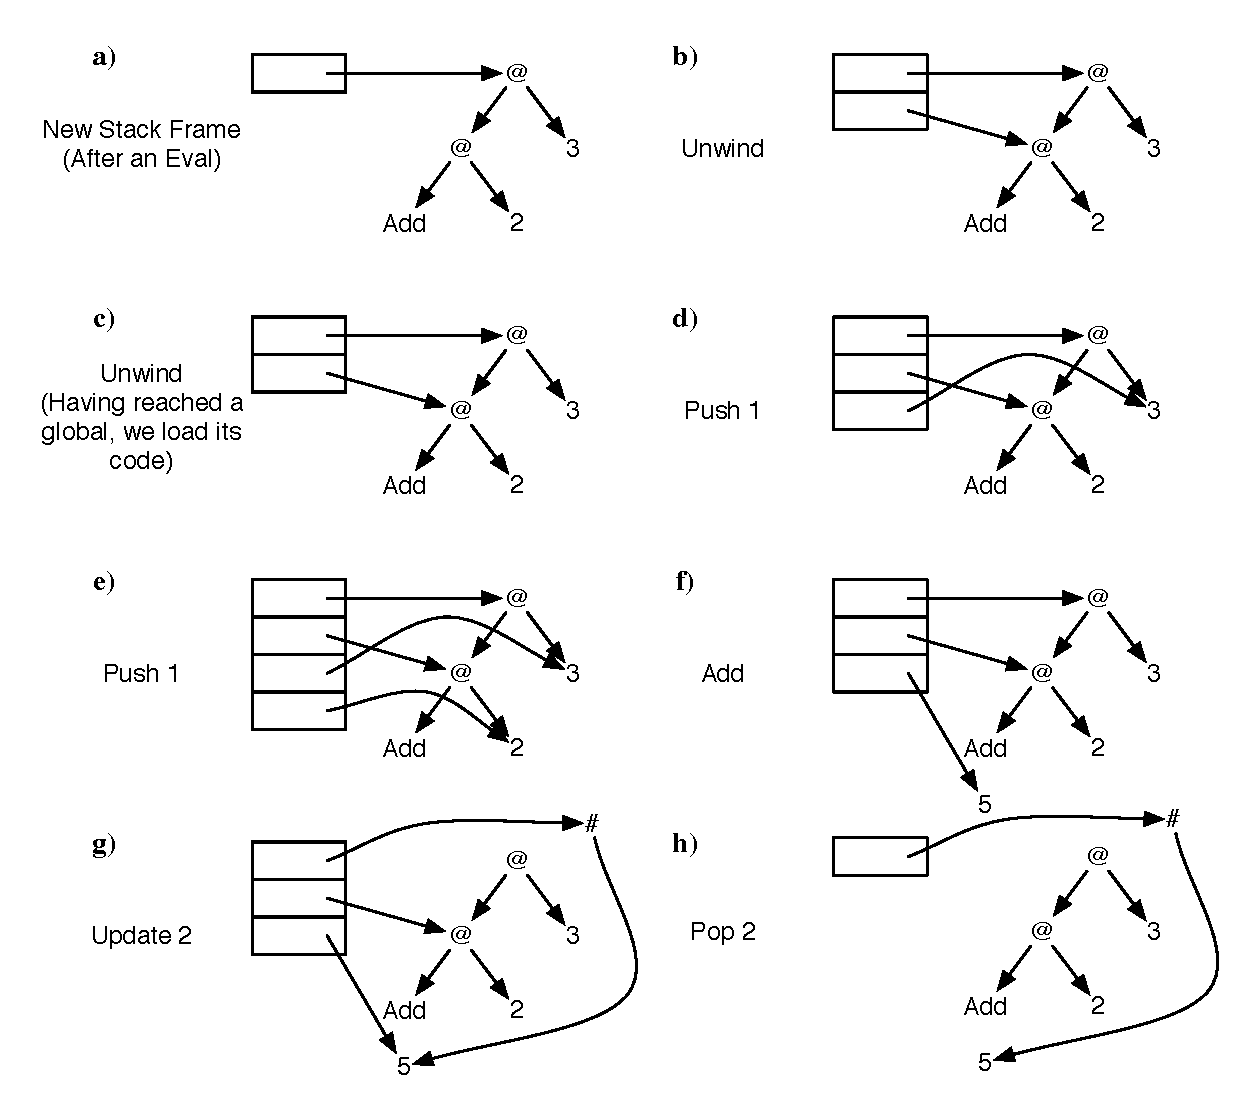
\includegraphics[scale=0.55]{Background/figures/AddExample.eps}
  \caption[G-Code execution example]
   {Walk-through of the \(G\)-Code for Add 2 3}
  \label{example:gCode}
\end{figure}

In figure \ref{example:gCode} we walk through a simple $G$-Machine reduction. 
At (a) we have we have a reduction about to take place, the top of the stack is
pointing to the root of the expression. In (b) the GCode instruction Unwind is
executed, placing a pointer to the application node's function argument on the
stack. Unwinding continues until a global function is encountered. 
When unwind reaches a global function, as in (c), the $G$-Machine loads
the code for that function and executes it. The code for \verb-Add- is Push 1,
Push 1, Add, Update 2, Pop 2, Unwind\footnote{This version of Add will only work
with primitives as its arguments. In order to accept expressions there would
need to be an Eval instruction added after every Push.}. 
The first three instructions are what
actually add the two arguments, with the last three instructions being used to
update the graph and begin unwinding again. Push 1 pushes a pointer to the
argument of the application node pointed to by the address located at stack
address 1 (the stack addressing starts at 0). This is done twice at (d)
and (e) in order to have pointers to both arguments at the top of the stack.
Then we have the Add instruction which dereferences the top two pointers and
adds the resulting values, the resulting value is then pushed onto the stack;
this is seen at (f). With the result now on the stack, updating takes place, (g). 
The Update instruction take a value (which is the arity of the function being
evaluated) and updates the stack pointer that originally pointed to the root of
the expression. The pointer is replaced by an indirection node, which is in turn
set to point to the same value as the top stack pointer. With the updating
finished the expression's original graph is no longer needed. Therefore, we can
pop all of the intermediate pointers on the stack, which will always be equal to
the arity of the expression. At (h) we are left with the updated pointer that
can now be used by the calling function. We execute the Unwind instruction again,
entering the $G$-Machine into its unwind state, which will ensure that the
proper stack jumping occurs when there is nothing left to evaluate (such as in
this case).

 \subsection{Spineless $G$-Machine}
    The standard $G$-Machine updates the shared graph after every reduction
step. While this is conceptually simple and easy to implement, such frequent
rewrites in the heap can be seen as wasteful. The Spineless
$G$-Machine improves on this by only updating the graph when loss of sharing is
a possibility \cite{burn1988spineless}. It is known as `spineless' because the 
chain of application nodes that would make up the spine in the standard 
$G$-Machine is not built up in the heap. Instead it is exclusively 
accumulated on the stack until an update is required. The key point in this
variation of the $G$-Machine is that updating should be associated with the
potential loss of sharing and not with a reduction \cite{burn1988spineless}.

    The way this was accomplished was by adding a new type of application node
which they call a ``SAP'' node (for shared application). A SAP node indicates
that the node is `updatable' and that the result of any reduction at that node
should be updated in the graph. 

    The mechanism for the updates is slightly different for functions than it is
for values. First let us look at how functions are handled. When a SAP node is 
pushed onto the stack during an unwinding a new stack frame is created. When a
pointer outside of the bounds of the stack frame is required we can take this as
a signal that the reduction occurring at the updatable node has resulted in a
function that `fails' the arity test. We then rewrite the subgraph at the SAP
node since we know that sharing could be lost if we continued otherwise.
For values the update is triggered when the value has been reduced to its
base-value form.

    The remaining task for the Spineless $G$-Machine is to determine which
application nodes should be a SAP node, and which should be a standard AP node. 
The authors give three different strategies for identifying which nodes should
be marked as SAP. The simplest strategy is that all nodes should be marked as
sharing nodes; this ensures that no sharing will be lost but will find the same
wasteful re-writing that the standard $G$-Machine exhibited. The next strategy
involves simple static sharing analysis to identify the nodes where the
arguments will definitely \emph{not} be shared, so all other nodes are marked as
sharing nodes. Lastly, a dynamic method is suggested that attempts to identify
as few sharing nodes as possible (therefore minimising the re-writing) while
adding an overhead cost of having to check when a shared subgraph is created.
The authors call this mechanism ``dashing'' and argue that the savings of having
as few re-writes as possible make the overhead cost of dashing worthwhile
\cite{burn1988spineless}.


 \subsection{STG-Machine}
    A few years after the design of the Spineless $G$-Machine, another
enhancement was introduced, the Spineless Tagless $G$-Machine. This descendant of
the $G$-Machine is a fully realised Spineless $G$-Machine that eliminates the
need for tagged nodes by using packets\footnote{The original terminology used
for this concept was either a closure, or a thunk; a thunk being a closure that
is fully saturated. However, to differentiate between the \emph{concept} of a
closure and its representation, a packet will refer to the STG-Machine's 
representation of a closure.} for its graph representation. 

    Each packet consists of a code pointer and zero or more pointer fields used
to point to the values of free variables. The code the packet points to is what
determines the behavior of the node. There is a global \emph{environment
pointer} which addresses a packet, and then the packets code is executed. If
there are any free variables associated with the packet the are accessed via an
offset from the environment pointer \cite{jones1992implementing}. This process
was called `entering' the packet. Because there is no tag on a node, the only
way of determining the purpose of the node is to enter the packet. As said by
Peyton Jones ``each closure (including data values) is represented uniformly,
and scrutinized only by entering it.'' \cite{jones1992implementing}. 

    The STG-Machine uses the self-updating model when having to update a
subgraph. Instead of updating after every reduction, like the $G$-Machine, each
packet is responsible for updating itself when an update is necessary. In the
case of a thunk, entering the packet will result in the thunk being overwritten
and the resulting packet's code will simply return the value stored in the
packet. 

    The STG-Machine became the basis for GHC and has had many improvements over
the years \cite{HistoryOfHaskell}. Interestingly, one of the improvements to the
STG-Machine was the introduction of tags! The elegance of being able to treat
every node the same has a cost on the performance on modern architectures
\cite{marlow2007faster}.
Because so much of the performance in modern CPUs comes from the speed of its
cache (and therefore avoiding the memory bottleneck) the indirections that arise
from the code pointers in each packet have a significant cost on performance. As
stated in the introduction to their 2007 paper \cite{marlow2007faster}:
\begin{quote}
The tagless scheme is attractive because the code to evaluate a closure is
simple and uniform: any closure can be evaluated simply by
entering it. But this uniformity comes at the expense of performing indirect
jumps, one to enter the closure and another to return to
the evaluation site. These indirect jumps are particularly expensive
on a modern processor architecture, because they fox the branchprediction
hardware, leading to a stall of 10 or more cycles depending on the length of the
pipeline. 
\end{quote}

As much as we would like to focus one elegant abstractions and distance
ourselves from the low level concerns, there will always be \emph{some} focus on
performance, and that will sometimes require compromises to accommodate hardware
realities. 

\section{Parallel Computation}
    Having looked at the $G$-Machine as a sequential abstract machine we can now
look at how graph reduction can occur on parallel architectures. The simplest
parallel variant would be a parallel $G$-Machine. It turns out that once
sequential graph reduction has been accounted for there is not much to add in
order to provide facilities for parallel evaluation. If one were to use a shared
graph almost all communication could take place via that graph.

\begin{figure}[hb]
  \centering
  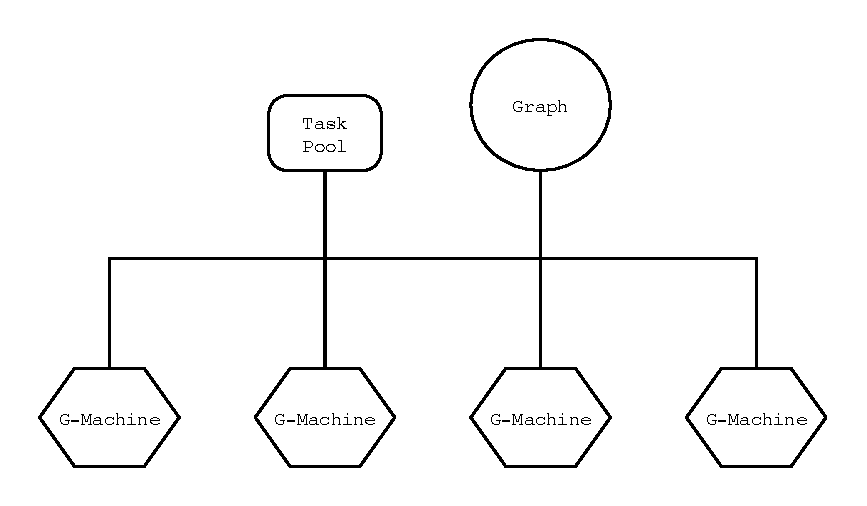
\includegraphics[scale=0.7]{Background/figures/simpleParallel.eps}
  \caption[Simple parallel graph reduction model]
   {A parallel G-Machine}
    \label{fig:simpleGMachine}
\end{figure}

The spark pool is where idle processors can look for subgraphs that have been
sparked off for evaluation. This simple-yet-functioning model is actually the
basis for the implementation described in chapter \ref{sec:implementation}
\cite{PeytonJones:1992:IFL:129390}.

 \subsection{$\langle \nu , G\rangle $-Machine}
    A departure from the stack-based approach of the G-Machine, here we have a
packet-based abstract machine \cite{vGMachine, Alice}. 
    The packets (or frame as they are called in the
original paper) are similar to the packets we have seen for the STG-Machine
(although the $\langle \nu , G\rangle $-Machine was described and implemented
first \cite{vGMachine}). One difference is that on top of the code pointer and
pointer to its arguments, there is a dynamic pointer that points to the caller of
the expression the packet represents, and there is a block of free `working
space' on each packet (we will see why in a moment). 
The key difference, however, is the way that the 
$\langle \nu , G\rangle $-Machine deals with its stack.
As opposed to having a central stack, each packet has its own, using the free
space allocated with the creation of the packet as its local stack.
Therefore the stack for a task is always in
the heap with the task itself \cite{vGMachine}. This is in contrast to the standard
G-Machine, where the stack resides `in' the machine itself and the tasks use
that stack until they are blocked, at which point the task's stack is
transferred to the heap until the task is awoken. 
    The $\langle \nu , G\rangle $-Machine avoids any complications of dealing
with the stack by distributing the stack amongst the graph. The stack frame at
any point in the graph is a accessed through the linked list of packets pointing
to their caller. 
    One possible way of thinking about this: The traditional stack-based approach has a
stack on each \emph{processor}, whereas the this approach has a stack on
each \emph{process}.
